\chapter{Der Detroit im aktuellen Zustand}\label{aktuell}

\textcolor{blue}{Dieses Kapitel soll vollständig über das Fahrzeug informieren, so wie es aktuell aufgebaut ist. Dabei werden modifizierte, aber auch im Originalzustand belassene Baugruppen erläutert. So sollen alle aktuellen Informationen zum \textsc{Detroit} zusammengefasst in diesem Kapitel zu finden sein.}

\section{Batterie}
Als Batterie für den \textsc{Detroit} sollten die modernen Lithium-Ionen-Akkumulatoren des Peugeot-Unfallfahrzeuges verwendet werden. Dabei wurden jedoch einige Anpassungen durchgeführt, da die Batterien zum einen nicht die selbe Spannung besassen, zum anderen beim \textsc{Detroit} auch zwei unabhängige Batterien verbaut waren. Dies zog umfangreiche Anpassungen mit sich, die nachfolgend erläutert werden.

\subsection{Funktion von Lithium-Ionen-Akkumulatoren} \label{kap_liion}

Lithium-Ionen-Akkumulatoren sind in der heutigen Zeit der Standard. Das heisst in allen neuartigen Handys, Mobiltelefonen aber auch in Fahrzeugen werden diese verbaut, wobei immer mehr auf Blei-Akkus verzichtet wird. Doch gibt es trotzdem Bereiche, in welchen Blei-Batterien immer noch ihre Anwendungen finden, wie zum Beispiel eine Starterbatterie in einem Auto. Die Technologie der Lithium-Ionen Akkus ist jedoch im Vergleich zu Blei-Batterien sehr jung, genauer gesagt ca. 50 Jahre alt, und hinter den effizienten Akkus liegt eine aufwändige Ladetechnik. Nachfolgend wird kurz die Funktionsweise und die Lade- / Entladekurve der Lithium-Ionen-Akkus erläutert.

\paragraph{Aufbau/Grundfunktion}
Der Name Lithium-Ionen-Akkumulator kommt von den Lithiumionen, die frei zwischen den beiden Elektroden wandern. Durch einen Separator sind die beiden Elektroden vor direktem Kontakt geschützt. Die positive Elektrode besteht aus Lithium-Metalloxiden wie zum Beispiel LiCoO$_2$, LiNiO$_2$ oder LiMn$_2$O$_4$ und die negative aus Graphit. Wichtig ist, dass die Elektrolytlösung frei von Wasser ist, damit sie nicht mit dem Lithium reagiert.
Grundsätzlich funktioniert der Akku so, dass während dem Ladevorgang positiv geladene Lithiumionen von der positiven zur negativen Elektrode übergehen und an der Kathode hängen bleiben. Gleichzeitig liefert der Ladestrom die Elektronen über eine von aussen angelegte Verbindung. Beim Entladevorgang ist die Funktion genau umgekehrt. Die Elektronen fliessen über den äusseren Stromkreis zur positiven Elektrode. Der Aufbau und die Grundfunktion sind in Figur \ref{fig:liion_akku} dargestellt \cite{liion_akku_aufbau_funktion2}:

\begin{figure}[h!]
	\centering
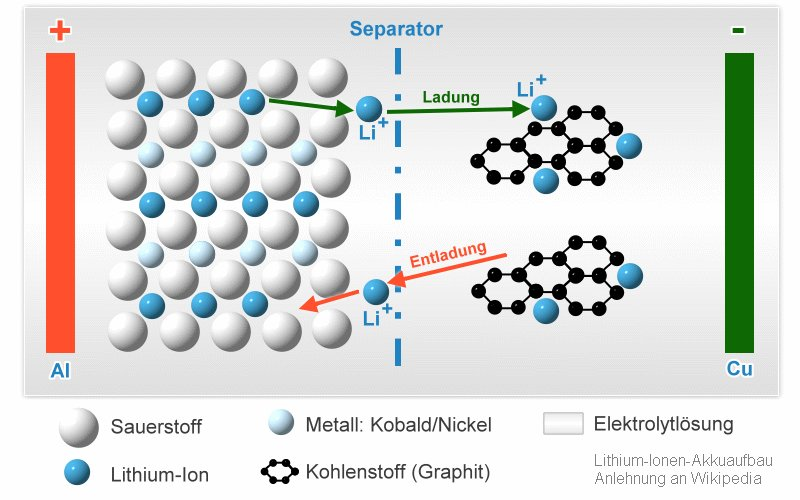
\includegraphics[width=0.74\textwidth]{images/aufbau_liion.jpg}
	\caption{Aufbau/Grundfunktion Lithium-Ionen-Akkumulator \cite{liion_akku_aufbau_funktion1}}
	\label{fig:liion_akku}
\end{figure}

\newpage

\paragraph{Lade-/Entladekurve}
Die typischen Lade-/Entladekurven sind nachfolgend in Abbildungen \ref{fig:liion_akku_ladekurve} und \ref{fig:liion_akku_entladekurve} aufgeführt:

\begin{figure}[h!]
	\centering
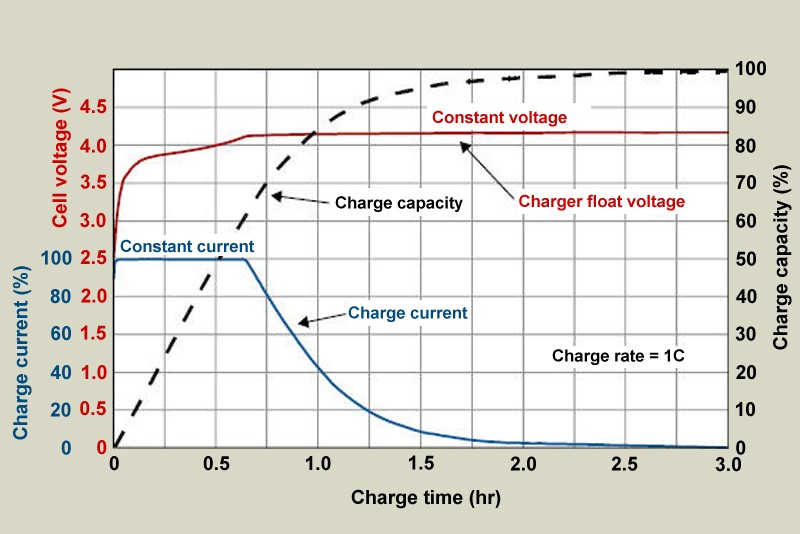
\includegraphics[width=1.0\textwidth]{images/liion_ladekurve.jpg}
	\caption{Ladekurve Lithium-Ionen-Akkumulator \cite{liion_ladekurve}}
\label{fig:liion_akku_ladekurve}
\end{figure}

\begin{figure}[h!]
	\centering
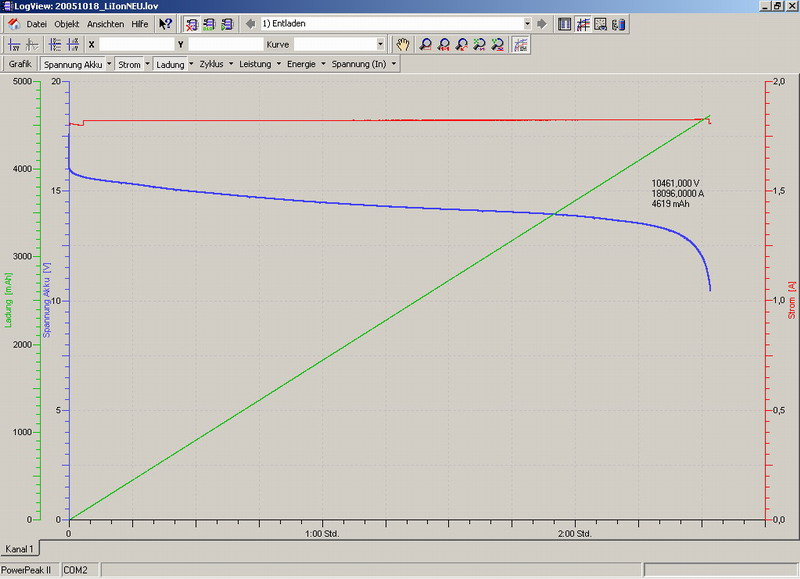
\includegraphics[width=1.0\textwidth]{images/liion_entladekurve.jpg}
	\caption{Entladekurve Lithium-Ionen-Akkumulator \cite{liion_entladekurve}}
\label{fig:liion_akku_entladekurve}
\end{figure}

\newpage

Beim Ladevorgang gemäss Abbildung \ref{fig:liion_akku_ladekurve} ist zu sehen, dass die Batteriespannung innert kurzer Zeit stark ansteigt. Anschliessend ist die Steigung flacher jedoch einigermassen linear. Am Ende wird der Ladestrom reduziert, wobei die Spannung konstant bleibt, bis 100\% der Kapazität erreicht wird.
Nahezu identisch funktioniert der Entladevorgang gemäss Abbildung \ref{fig:liion_akku_entladekurve} jedoch einfach umgekehrt. Die Spannung ist über einen weiten Zeitraum linear und erst am Ende bricht sie zusammen. Eine ähnliche jedoch gespiegelte Kurve kann beim Entladevorgang beobachtet werden.
Zu erwähnen ist noch, dass es sich bei den beiden Figuren in den Abbildungen \ref{fig:liion_akku_ladekurve} und \ref{fig:liion_akku_entladekurve} um unterschiedliche Verschaltungen der Batterien handelt und somit auch um unterschiedliche Ladebereiche. Aus diesem Grund sind auch die Spannungen unterschiedlich, jedoch bleibt die Form der Kurven gleich. Diese Kurve hat somit zwei Stufen: Zuerst wird der Strom begrenzt, damit die thermische Belastung verhindert wird. Danach wird die Spannung begrenzt, damit diese nicht weiter steigt und die Batterien zerstören könnte. Beim Laden wird sie nach oben begrenzt, da sich der Akku sonst aufbläht. Beim Entladen wird die Spannung nach unten begrenzt, da sonst Tiefentladung entstehen könnte. Wobei der Strom immer durch die Anwendung begrenzt werden sollte, da der Innenwiderstand sehr klein ist.

\newpage

\subsection{Vergleich Blei / Lithium-Ionen} \label{kap:Vergleich_liion_pb}

Um die Unterschiede von Lithium-Ionen zu Blei-Akkus besser zu verstehen, sind nachfolgend kurz einige Vor- und Nachteile aufgelistet. Zusätzlich sind in Tabelle \ref{tab:Vergleich} einige Vergleiche dargestellt.

\paragraph{Vorteil Blei}

Kurzfristige Lieferung von hohen Strömen ist für Blei-Akkumulatoren kein Problem. Sie besitzen ein gutes Preis-/Leistungsverhältnis und sind sehr zuverlässig, wenn Wartung und Pflege eingehalten werden. Ebenfalls sind sie relativ einfach in der Ladetechnik.

\paragraph{Nachteil Blei}

Die Energiedichte ist sehr gering. Das heisst, es braucht ein grosses Volumen und somit ein hohes Gewicht, um überhaupt ansatzweise eine gute Kapazität zu erreichen. Auch ist das Elektrolyt säurehaltig, womit Verätzungsgefahr besteht. Zusätzlich können normale Blei-Akkus nur waagerecht gelagert oder verbaut werden, da sonst das schädliche Elektrolyt auslaufen würde.

\paragraph{Vorteil Lithium-Ionen}

Der Akku besitzt eine sehr hohe Energiedichte, was auch für das geringe Gewicht der Akkumulatoren verantwortlich ist. Ebenfalls sind die Akkumulatoren sehr lange haltbar und müssen selten ausgetauscht werden. Auch ist es möglich diese über Monate aufzubewahren, ohne grosse Einbussen in der Ladung zu bemerken.

\paragraph{Nachteil Lithium-Ionen}

Eine aufwändige Ladetechnik und ein Batteriemanagementsystem, kurz BMS, wird benötigt, da die Batterien sehr heikel gegenüber Über- und Unterspannung und auch Übertemperatur reagieren. Somit kommen zusätzliche Kosten hinzu.

\paragraph{Lade-/Entladekurven}

Beide Kurven (siehe Abbildungen \ref{fig:pb_akku_kurve} und \ref{fig:liion_akku_ladekurve}/\ref{fig:liion_akku_entladekurve}) weisen sowohl Gemeinsamkeiten als auch Unterschiede auf. Beide Akkus werden mit dem CCCV(Constant-Current / Constant-Voltage)-Verfahren  geladen. Das bedeutet beim Laden konstanter Strom, bis ein kritischer Punkt in der Spannung erreicht wird. Dann wird die Spannung konstant gehalten um den Strom zu reduzieren. Das Gleiche passiert beim Entladevorgang, einfach umgekehrt. Zu erwähnen ist, dass Lithium-Ionen hier extrem empfindlich sind, wobei mit Blei-Akkus ein wenig gespielt werden kann, ohne dass diese zerstört werden.

\newpage

\begin{table}[h!]
\centering
\begin{tabular}{|l|l|l|}
\hline
\textbf{Akkutyp}                  & \textbf{Bleiakku}                                                                  & \textbf{Lithium-Ionen-Akku}                                                                   \\ \hline
Energiedichte in Wh/kg   & 30-40                                                                     & 70-200                                                                        \\ \hline
(Nenn) Zellspannung      & 2.0 V                                                                     & 3.7 V                                                                         \\ \hline
Ladewirkungsgrad         & 80-85\%                                                                   & 90-95\%                                                                       \\ \hline
Lebensdauer des Akkus    & \begin{tabular}[c]{@{}l@{}}5-15 Jahre\\ \textless3000 Zyklen\end{tabular} & \begin{tabular}[c]{@{}l@{}}15-25 Jahre\\ \textgreater5000 Zyklen\end{tabular} \\ \hline
Selbstentladung im Monat & 5-10\%                                                                    & 1-2\%                                                                         \\ \hline
Preis in Fr/kWh          & 500                                                                       & 800                                                                           \\ \hline
Temperaturbereich ideal  & 15-40$^\circ$C                                                            & 10-40$^\circ$C                                                                \\ \hline
\end{tabular}
\caption{Vergleichswerte Blei - Lithium-Ionen \cite{vergleich_liion_pb}}
\label{tab:Vergleich}
\end{table}

\paragraph{Fazit}

Beide Akkutypen haben ihre Vor- und Nachteile und es kommt stark auf die Anwendung der Batterie an. Für Starterbatterien in einem normalen Auto kann ohne Probleme eine günstige Blei-Batterie verwendet werden, da diese ohne Probleme kurzzeitig einen hohen Startstrom liefern kann. Wenn jedoch wie in unserem Fall ein Fahrzeug dauerhaft mit Akkumulatoren läuft, ist es sinnvoll auf das Gewicht bzw. Lebensdauer und nicht auf den Preis zu achten und somit sind Lithium-Ionen-Batterien hier definitiv die bessere Wahl.